\section{Phương pháp giải toán}

Trong phần này, báo cáo kỹ thuật trình bày tổng quan phương pháp đề xuất cho tác vụ nhúng đồ thị tri thức và tối ưu hóa mô hình. Chúng tôi cũng điểm lại những khái niệm cơ sở của học tăng cường trong ngữ cảnh dữ liệu đa quan hệ như đồ thị tri thức.

\subsection{Tổng quan phương pháp}

\begin{sidewaysfigure}
    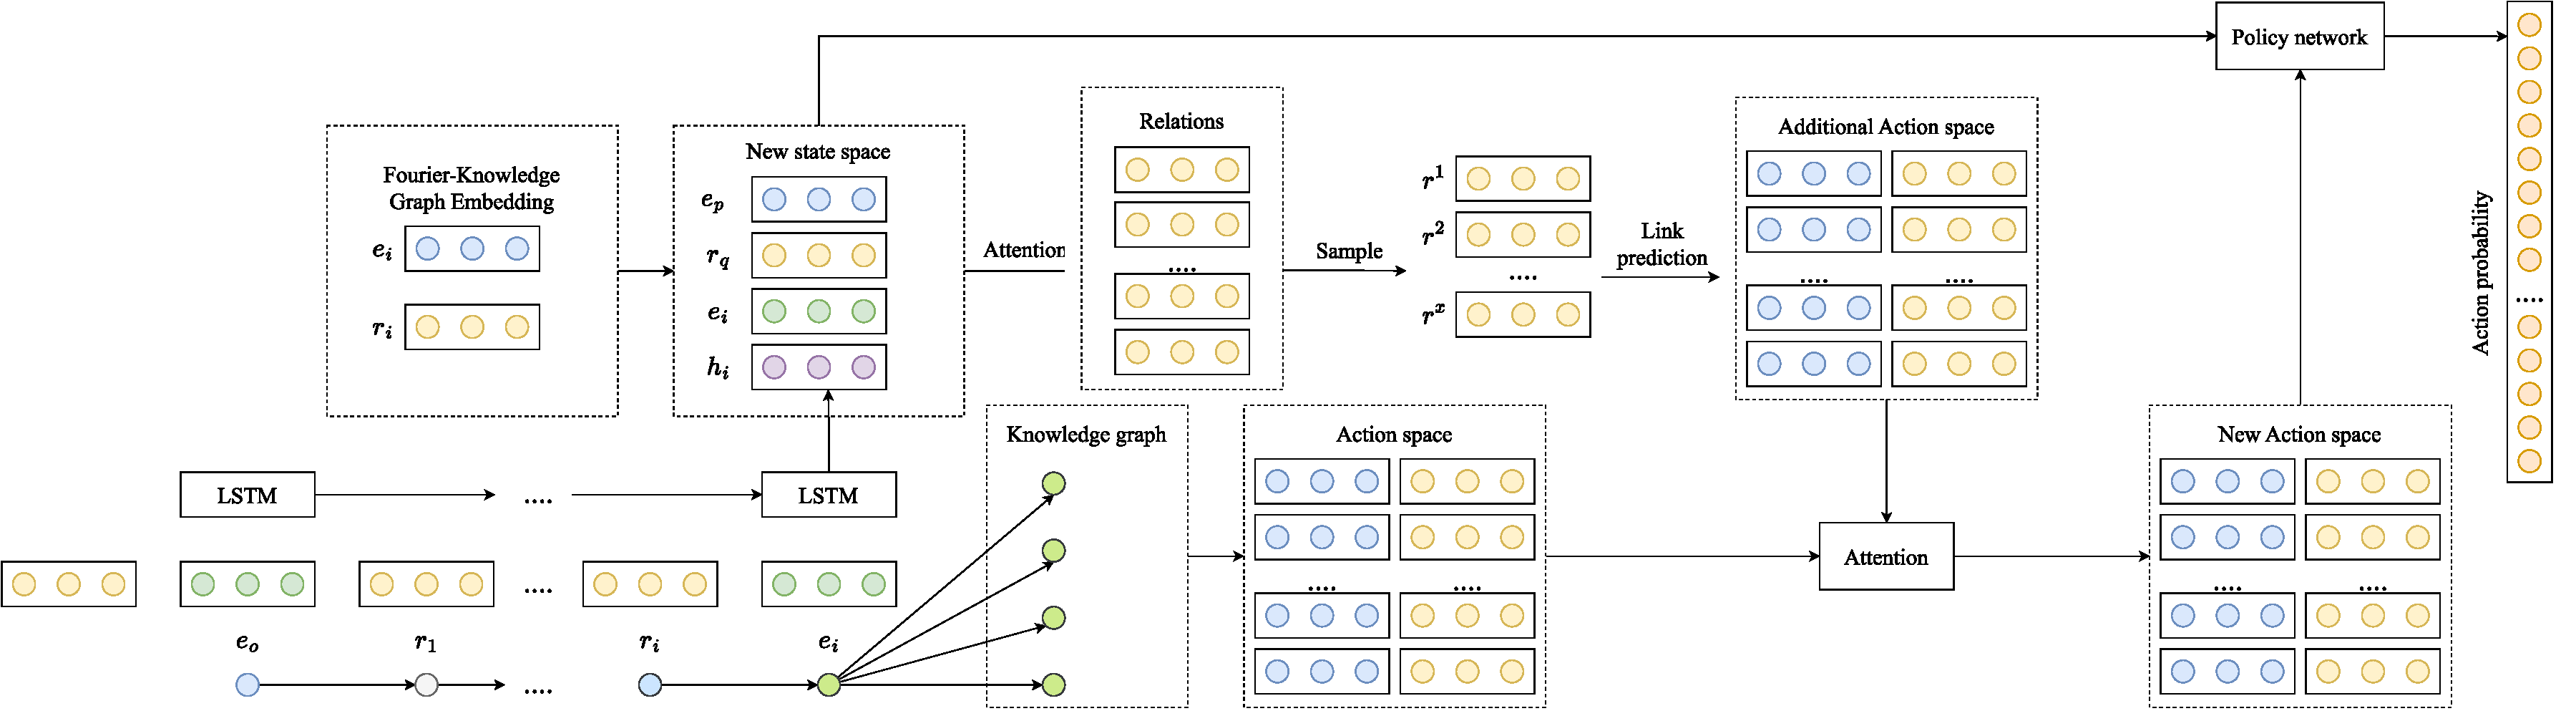
\includegraphics[width=1.\linewidth]{rl_framework.pdf}
    \caption{Tổng thể kiến trúc RL framework đề xuất.}
    \label{fig:rl_frame_arch}
\end{sidewaysfigure}


\subsection{Fourier-Knowledge Graph Embedding}

Lấy động lực từ việc mô hình ComplEx không có khả năng mô hình hóa các bộ ba dữ kiện với những quan hệ bắc cầu (transitive relation)
do đó mô hình này chưa thật sự tốt trên các bộ dữ liệu thực nghiệm, điều này được chỉ ra trong bài báo của Sun et al.\cite{sun2019rotate}.
Trong báo cáo kỹ thuật này, chúng tôi đề xuất sử dụng phép biến đổi Fourier trong không gian số phức, gọi là Fourier-Knowledge Graph Embedding (Fkge)
nhằm cải thiện hiệu quả của mô hình pretrain-KGE cho Reinforcement Learning framework để giải quyết bài toán suy diễn đồ thị tri thức đa bước.

Cho trước một bộ ba dữ kiện $(h, r, t)$, gọi các embedding vectors của chúng lần lượt là $(\mathbf{h}, \mathbf{r}, \mathbf{t})$ trong không gian phức. 
Hàm tính điểm của $\text{Fkge}: \mathbb{C}^{3d} \rightarrow \mathbb{R}$:

\begin{equation}
    \text{Fkge}(\mathbf{h}, \mathbf{r}, \mathbf{t}) = \sigma(\text{rfft}\left(\frac{1}{2}\left(\text{max}(\text{irfft}(\mathbf{h}), Re(\mathbf{r})) + \text{min}(\text{irfft}(\mathbf{h}), Im(\mathbf{r}))\right)\right) \circ \mathbf{t})
\end{equation}
trong đó:
\begin{itemize}
    \item $\sigma$: là hàm kích hoạt phi tuyến, ở đây sử dụng hàm sigmoid
    \item $\text{rfft}$: phép biến đổi Fourier thực thuận
    \item $\text{rifft}$: phép biến đổi Fourier thực nghịch
\end{itemize}

Để mà huấn luyện mô hình nhúng đồ thị, chúng tôi sử dụng hàm mất mát lấy mẫu âm với chiến lược self-adversarial training\cite{sun2019rotate} như sau:

\begin{equation}
    \mathcal{L} = -log(\sigma(\lambda - \text{Fkge}(\mathbf{h}, \mathbf{r}, \mathbf{t})) - \sum_{i=1}^np(\mathbf{h}', \mathbf{r}', \mathbf{t}')log(\sigma(\text{Fkge}(\mathbf{h}, \mathbf{r}, \mathbf{t}) - \lambda))
\end{equation}
trong đó: $\lambda$ là siêu tham số lề (margin) cho trước.

Với những mẫu âm, chúng được lấy mẫu dựa trên phân phối được định nghĩa như sau:
\begin{equation}
    p(\mathbf{h}_j', \mathbf{r}, \mathbf{t}_j' \mid \mathbf{h}_k, \mathbf{r}, \mathbf{t}_k) = \frac{\text{exp}(\alpha\text{Fkge}(\mathbf{h}_j', \mathbf{r}, \mathbf{t})_j')}{\sum_{k=1}\text{exp}(\alpha\text{Fkge}(\mathbf{h}_k', \mathbf{r}, \mathbf{t})_k'))}
\end{equation}
trong đó: $\alpha$ lả hệ số nhiệt lượng lấy mẫu (temperature of sampling)


\subsection{Khung học tăng cường cho suy diễn đa bước}

Trong phần này, chúng tôi định nghĩa lại những khái niệm cơ sở của Markov Decision Process (MDP) trong mô hình suy diễn đồ thị tri thức đa bước.

\subsubsection{Không gian trạng thái (state space)}

Không gian hành động trong suy diễn đồ thị tri thức đa bước có thể được định nghĩa từ quan hệ
mục tiêu (target relation), nút hiện tại (current node) và các đường đi lịch sử (historical paths).
Trạng thái của bước thứ $i$ có thể được định nghĩa:

\begin{equation}
    s_i = (r_q, e_i, h_i)
\end{equation}
trong đó: $r_q$, $e_i$, và $h_i$ lần lượt là các vector đặc trưng của quan hệ, thực thể, và đường đi lịch sử tương ứng.

Trong quá trình suy diễn đa bước, cạnh (quan hệ) mà tác tử lựa chọn không chỉ phụ thuộc vào quan hệ $\textbf{r}_q$ và thực thể hiện tại $\textbf{e}_i$, mà còn
phụ thuộc vào những đường đi ở trong quá khứ. Dựa trên điều này, chúng tôi sử dụng LSTM để mã hóa thông tin $\textbf{h}_i$.

Dựa trên phát hiện của Das et al., Lin et al., về hiện tượng các mô hình KGE không phụ thuộc vào tính liên thông của đồ thị tri thức. Bằng cách sử dụng mô hình KGE được huấn luyện từ trước, vector xác suất của tất cả thực thể đuôi. Một cách cụ thể,
ta gọi vector xác suất $\mathbf{p} \in \mathbf{R}^{|\mathcal{E}|}$, trong đó giá trị của chiều thứ $i$ thể hiện xác suất mà $e_i$ là thực thể đuôi đúng.
Chiến lược dynamic anticipation được đề xuất bởi Lv et al.\cite{lv2020dynamic} cho phép ta thay đổi công thức thể hiện trạng thái như sau:

\begin{equation}
    \mathbf{s}_i = (\mathbf{e}_p, \mathbf{r}_q, \mathbf{e}_i, \mathbf{h}_i)
\end{equation}
trong đó: $\mathbf{e}_p$ là thông tin dự đoán được từ mô hình KGE.

\subsubsection{Không gian hành động (action space)}

Với $s_i = (r_q, e_i, h_i)$, nếu tồn tại một bộ ba dữ kiện $(e_i, {r}_n, {e}_n)$ trong đồ thị
tri thức, ta có thể xem $({r}_n, {e}_n)$ là một trong các hành động, nhiều hành động tạo nên không gian hành động của tác tử. Thế nên, không gian 
hành động của tác tử trong trạng thái hiện tại được định nghĩa:

\begin{equation}
    \mathcal{A}_i = \{({r}_n, {e}_n) \mid ({e}_i, {r}_n, {e}_n) \in \mathcal{T}\}
\end{equation}
trong đó: $\mathcal{T}$ thể hiện cho tất cả bộ ba dữ kiện của đồ thị tri thức. Để đảm bảo rằng tác tử có thể dừng được trong quá trình suy diễn,
các khuyên $({r}_{loop}, {e}_i)$ cũng được thêm vào dữ liệu đồ thị. Đây có thể xem như là một kỹ thuật tăng cường dữ liệu.

Chúng tôi kết hợp phương pháp Dynamic Completion được đề xuất bởi Lv et al.\cite{lv2020dynamic}, và phương pháp được đề xuất bởi Zhou et al.\cite{zhou2021multi}
để tăng cường không gian hành dộng cho mô hình. Ta gọi tập hợp các hành động bổ trợ (additional actions) 
$C_i = \{(r, e) | \in \mathcal{R} \wedge e \in \mathcal{E} \wedge (e_i, r, e) \notin \mathcal{T}\}$. Ta sẽ chọn những hành động
với xác suất cao từ $C_i$, xác suất này có thể được định nghĩa:

\begin{equation}
    p((r, e) \mid s_i) = p(r \mid s_t)p(e \mid r, s_i)
\end{equation}

Để tối ưu hóa thời gian trong việc lập trình, ta lựa chọn một số quan hệ với xác suất cao bằng cách dùng $p(r \mid s_t)$, sau đó 
chọn những quan hệ với xác suất cao cho một số quan hệ đã chọn này bằng $p(e \mid r, s_t)$

Với trạng thái hiện tại, ta tính được giá trị attention trên tất cả các quan hệ $p(r \mid s_t)$,

\begin{equation}
    \mathbf{w} = \text{softmax}(\text{MLP}(\mathbf{s}_i) \dot [\mathbf{r}_1, ..., \mathbf{r}_\mathcal{R}])
\end{equation}

Kích thước của không gian hành động của trạng thái hiện tại được kiểm soát bởi tham số $\alpha$ và số lượng hành động cực đại $M$

\begin{equation}
    N_{add} = min([\alpha N], M)
\end{equation}

Sau đó, chọn $x$ quan hệ với giá trị attention lớn nhất trong $\mathbf{w}$ để hình thành một tập quan hệ mới $\mathcal{R}_{add} = \{r^1, r^2, ..., r^x\}$. 
Với một mô hình KGE được huấn luyện sẵn, không gian hành động bổ trợ được định nghĩa:

\begin{equation}
    \mathcal{A}_i^{add} = \{(r^i, e_{r^i}^1), ..., (r^k, e_{r^k}^1)\}
\end{equation}

Để hình thành không gian hành động mang ngữ nghĩa tốt hơn, cơ chế attention được tiếp tục sử dụng:

\begin{equation}
    \mathcal{A}_i = \text{Attention}(\mathcal{A}_i, \mathcal{A}_i^{add}, [\mathcal{A}_i;\mathcal{A}_i^{add} ])
\end{equation}

\subsubsection{Xác suất dịch chuyển trạng thái (transition)}

Nếu trạng thái hiện tại là $s_i = (r_q, {e}_i, {h}_i)$, và tác tử chọn hành động tiếp theo là $({r}_n, {e}_n) \in \mathcal{A}_i$,
thì trạng thái hiện tại $s_i$ sẽ bị biến đổi thành trạng thái kế tiếp 

\begin{equation}
    s_{i+1} = ({r}_q, {e}_n, {h}_{i+1})
\end{equation}

Trong lập trình, chúng ta sẽ phải giới hạn số bước về $T$, và xác suất chuyển ở bước cuối cùng sẽ là

\begin{equation}
    {s}_T = ({r}_q, {e}_T, {h}_{T})
\end{equation}

\subsubsection{Phần thưởng (reward)}

Với một truy vấn cho trước $({e}_s, {r}_q, ?)$, gọi đáp án truy vấn chính xác là ${e}_o$. Nếu tác tử dừng
tại thực thể chính xác ấy, tức là ${e}_T = {e}_o$, thì phần thưởng (reward) lúc này bằng 1. Ngược lại, 
phần thưởng có giá trị trong khoảng từ 0 đến 1 với hàm tính toán $f({e}_s, {r}_q, {e}_T)$, trong đó $f(.)$ 
là một hàm của một mô hình nhúng đồ thị tri thức (knowledge graph embedding - KGE) được huấn luyện trước để đánh giá tính hợp lý của
bộ ba $({e}_s, {r}_q, {e}_T)$

\subsubsection{Mạng chính sách (policy network)}

Để có thể hướng dẫn tác tử chọn hành động đúng đắn trong không gian các hành động khác nhau,
một mạng chính sách (policy network) là cần thiết. Tổng quan kiến trúc Policy network được thể hiện trong Hình \ref{fig:policy_network_arch}

Các đối tượng trong đồ thị tri thức bao gồm các thực thể và quan hệ được thể hiện như những vectors trong không gian
ngữ nghĩa, và một hành động $({r}_i, {e}_i)$ tại bước $t$ có thể được biểu diễn như 
$\mathbf{a}_i = [\textbf{r}_i, \textbf{e}_i]$, trong đó $\textbf{r}_i$ và $\textbf{e}_i$ là các vector của $r_i$ và $e_i$ tương ứng.

Để mã hóa thông tin đường đi quá khứ, mô hình LSTM (Long-short term memory) được sử dụng. Một cách cụ thể,
thể hiện của mỗi hành động được chọn bởi tác tử sẽ được đưa vào LSTM để sinh ra thông tin đường đi quá khứ.

\begin{equation}
    \mathbf{h}_i = \text{LSTM}(\mathbf{h}_{i-1}, \mathbf{a}_{i-1})
\end{equation}

Biểu diễn trạng thái thứ $i$: $s_i = (r_q, e_i, h_i)$

\begin{equation}
    \mathbf{s}_i = [\mathbf{r}_q, \mathbf{e}_i, \mathbf{h}_i]
\end{equation}

Hình thành ma trận hành động $\mathbf{A}_t \in \mathbb{R}^{|\mathcal{A}_t| \times 2d}$,
trong đó $d$ là chiều của các vector nhúng thực thể và quan hệ.

Mạng policy được định nghĩa:

\begin{equation}
    \pi_0(a_t | s_t) = \sigma(\mathbf{A}_t(\mathbf{W}_1\text{ReLU}(\mathbf{W}_2\mathbf{s}_t)))
\end{equation}
trong đó: $\sigma$ là toán tử softmax, $\mathbf{W}_1$ và $\mathbf{W}_2$ là các ma trận biến đổi tuyến tính (linear neural network),
và $\pi_0(a_t | s_t)$ là phân phối xác suất trên tất các hành động trong $\mathcal{A}_t$

\begin{center}
    \centering
    \begin{figure}[h!]
        \includesvg[scale=0.4]{policy_network.svg}
        \caption{Kiến trúc Policy network.}
        \label{fig:policy_network_arch}
    \end{figure}
\end{center}

\subsection{Tối ưu hóa cho khung học tăng cường}

Trong phần này, chúng tôi trình bày kỹ thuật tối ưu cho RL Learning framework. Một cách cụ thể, chúng tôi sử dụng các phương pháp tối ưu bậc nhất
thích nghi dựa trên local model:
\begin{itemize}
    \item Phương pháp Adaptive Moment Estimation (Adam):  Là một phương pháp tối ưu hóa thường được sử dụng trong huấn luyện các mạng học sâu. 
    Ý tưởng đằng sau Adam là tính toán những tỉ lệ học cho từng tham số dựa trên ước lượng bậc nhất và bậc hai moment của gradients.
    \item Phương pháp Quasi-Hyperbolic Momentum: QHM là một phương pháp cải tiến dựa trên các phương pháp momentum truyền thống. Nó thêm vào một phân số
    của cập nhật trước đó cho cập nhật hiện tại để giúp tối ưu di chuyển hơn, nhanh hơn theo hướng của gradient. Tác dụng của phân số này giúp cho sự cân bằng của 
    cập nhật trước đó và hiện tại trở nên cân bằng hơn. Điều này được thực hiện bằng việc sử dụng hypergradient như một siêu tham số kiểm soát tính cân bằng.
\end{itemize}

\subsubsection{Phương pháp Adaptive Moment Estimation}

Adaptive Moment Estimation Method hay Adam cũng thích ứng learning rate đến mỗi tham số. Nó lưu giữ cả mức giảm trung bình cấp số nhân giống như RMSProp và AdaDelta, và cả mức giảm gradient cấp số nhân như momentum. Nói một cách khác, Adam là một phương pháp tận dụng những lợi thế của những bộ tối ưu đi trước.

Khởi tạo gradient và gradient bình phương về 0 dẫn đến sai lệch. Một cài đặt tinh chỉnh bias giúp giảm bớt các vấn đề và theo bài báo gốc, $\alpha = 0,001 $, $ \gamma_v = 0,9 $, $ \gamma_s = 0,999 $ và $ \epsilon = 1 \times 10 ^ {- 8} $. Các bước cập nhật cho thuật toán diễn ra như sau trong quá trình huấn luyện mạng học sâu:

1) Cập nhật ước lượng momentum có thiên vị.

\begin{equation}
    \mathbf{v}^{(k+1)} = \gamma_v\mathbf{v}^{(k)} + (1-\gamma_v)\mathbf{g}^{(k)}
\end{equation}

2) Cập nhật ước lượng gradient có thiên vị.

\begin{equation}
    \mathbf{s}^{(k+1)} = \gamma_s\mathbf{s}^{(k)} + (1-\gamma_s)\left(\mathbf{g}^{(k)} \odot \mathbf{g}^{(k)}\right)
\end{equation}

3) Tính toán hiệu chỉnh ước lượng momentum có thiên vị.

\begin{equation}
    \hat{\mathbf{v}}^{(k+1)} = \mathbf{v}^{(k+1)} / (1-\gamma_v^k)
\end{equation}

4) Tính toán hiệu chỉnh ước lượng gradient có thiên vị.

\begin{equation}
    \hat{\mathbf{s}}^{(k+1)} = \mathbf{s}^{(k+1)} / (1-\gamma_s^k)
\end{equation}

5) Cập nhật tham số

\begin{equation}
    \mathbf{x}^{(k+1)} = \mathbf{x}^{(k)} - \alpha\hat{\mathbf{v}}^{(k+1)} / \left(\epsilon + \sqrt{\hat{\mathbf{s}}^{(k+1)}}\right)
\end{equation}

\subsubsection{Phương pháp Quasi-Hyperbolic Momentum \& Adam}

QHM (Quasi-Hyperbolic Momentum) là một thuật toán momentum thích ứng khác mà tách momentm ra khỏi gradient hiện tại khi cập nhật trọng số. Nói một cách khác, nó là trung bình có trong số của momentum và SGD đơn giản, tính theo gradient hiện tại với discount factor tức thời. Công thức cập nhật của Quasi-Hyperbolic Momentum có thể biến đổi trở về để suy biến trổ về Nesterov Momentum, Synthesized Nesterov Variants, accSGD và một số trường hợp khác. Luật cập nhật của thuật toán như sau:

\begin{equation}
    \mathbf{v}^{(k+1)} = \beta\mathbf{v}^{(k)} + (1-\beta) \cdot \mathbf{g}^{(k)}
\end{equation}

\begin{equation}
    \mathbf{x}^{(k+1)} = \mathbf{x}^{(k)} - \alpha \left[(1-\nu) \cdot \mathbf{g}^{(k)} + \nu \cdot \mathbf{v}^{(k+1)}\right]
\end{equation}
trong đó các hệ số $\nu = 0.7$ và $\beta = 0.999$


